\chapter{Технологическая часть}

\section{Средства написания программы}
Для реализации программного обеспечения были использованы следующие средства:

\begin{itemize}
    \item cреда разработки PyCharm 2023 community edition \cite{lib:pycharm};
    \item язык разработки Python 3.12 \cite{lib:python}.
\end{itemize}
	
Используемые библиотеки:
\begin{itemize}
    \item gymnasium — предоставляющая интерфейс для работы со средой \cite{lib:gymnasium};
    \item gymnasium\_robotics — предоставляющая среду AdroitHandHammer-v1 \cite{lib:gymnasium_robotics};
    \item stable\_baselines3 — библиотека для реализации алгоритмов машинного обучения, в частности PPO \cite{lib:stable_baselines3};
    \item numpy — для быстрой работы с массивами, сохранения промежуточных данных и связи их с другими библиотеками \cite{lib:numpy};
    \item matplotlib.pyplot — для отображения графиков \cite{lib:matplotlib};
    \item pathlib.Path — доступ к файлам системы \cite{lib:pathlib}.
\end{itemize}

\section{Программная реализация}

\begin{lstlisting}[label=init, caption={Инициализация}]
import gymnasium as gym
import gymnasium_robotics
from gymnasium.wrappers import RecordVideo
import matplotlib.pyplot as plt
import numpy as np
from pathlib import Path
from stable_baselines3 import PPO
from stable_baselines3.common.callbacks import BaseCallback
WORK_DIR = Path.cwd().resolve()
IMG_DIR = WORK_DIR / "report" / "images"
VID_DIR = WORK_DIR / "video"
env = gym.make('AdroitHandHammer-v1', render_mode="rgb_array")
env = RecordVideo(env, str(VID_DIR), episode_trigger=lambda e: True)
device = "cuda" if torch.cuda.is_available() else "cpu"
\end{lstlisting}
Этот код выполняет подготовительные действия для обучения модели с подкреплением. 
Сначала подключаются необходимые инструменты.

Затем определяются пути к рабочим директориям, где будут сохраняться изображения и видео. 
Создается среда обучения под названием AdroitHandHammer-v1, 
в которой агент будет управлять роботизированной рукой, чтобы забить гвоздь молотком. 
Среда настраивается таким образом, чтобы можно было получать визуальное представление происходящего в виде изображения.
Дополнительно включается запись видео, причем записываться будет каждый эпизод взаимодействия агента со средой.
Наконец, определяется, какое устройство будет использоваться для вычислений: графический процессор, если он доступен, или центральный процессор в противном случае.

\begin{lstlisting}[label=init, caption={Обучение модели и настройки колбэка}]
    class TrainingMonitorCallback(BaseCallback):
        def __init__(self, verbose=0):
            super().__init__(verbose)
            self.rewards = []
        def _on_step(self) -> bool:
            if "rewards" in self.locals:
                self.rewards.append(self.locals["rewards"])
            return True
    model = PPO("MlpPolicy", env, verbose=1, device=device)
    callback = TrainingMonitorCallback()
    total_timesteps = 1000000
    model.learn(total_timesteps=total_timesteps, callback=callback)
    model.save("ppo_adroit_hammer")
\end{lstlisting}
Создается колбэк, предназначенный для сбора данных о наградах (rewards) в процессе обучения.
Модель PPO с политикой \textit{MlpPolicy} обучается в среде env в течение 1 000 000 временных шагов. 
Колбэк \textit{TrainingMonitorCallback} добавляется в процесс обучения для мониторинга.
На каждом шаге обучения колбэк проверяет наличие переменной \textit{rewards} в локальных переменных и, 
если она существует, добавляет ее значение в список.
После завершения обучения модель сохраняется в файл \textit{ppo\_adroit\_hammer}. 

\begin{lstlisting}[label=init, caption={Тестирование}]
    obs, _ = env.reset()
    while True:
        action, _ = model.predict(obs, deterministic=True)
        obs, reward, done, truncated, _ = env.step(action)
        print(f"REWARD: {reward}")
        if done or truncated:
            obs, _ = env.reset()
            break
\end{lstlisting}
Окружение сбрасывается в начальное состояние.
Начинается цикл взаимодействия модели с окружением, который продолжается до тех пор, 
пока эпизод не завершится или не будет прерван.
Модель, на основе текущего наблюдения, предсказывает действие. 
Выбранное действие применяется в среде. 
Метод \textit{step} возвращает новое наблюдение, награду, флаги завершения и прерывания.
Значение полученной награды выводится на печать.
Если эпизод завершился или был прерван, среда сбрасывается, и цикл прерывается.

\section{Результаты}

График \ref{fig:training_rewards} демонстрирует успешное обучение модели PPO в среде AdroitHandHammer-v1. 
Начав с периода исследования и низких наград, агент постепенно вырабатывает эффективную стратегию, 
что отражается в значительном и продолжительном росте суммарной награды на протяжении большей части процесса обучения. 
Это свидетельствует о том, что модель научилась успешно управлять рукой-роботом для выполнения задачи забивания гвоздя.

Рисунки \ref{fig:work1} и \ref{fig:work2} демонстрируют, как агент успешно применяет полученную стратегию для выполнения задачи.

\begin{figure}[H]
    \centering
    \includegraphics[width=1\textwidth]{C:/MGTU/baseAI/lr12/lr12/bag/report/images/training\_rewards.png}
    \caption{Полученные награды в процессе обучения}
    \label{fig:training_rewards}
\end{figure}

\begin{figure}[H]
    \centering
    \begin{minipage}[H]{0.49\linewidth}
        \centering
        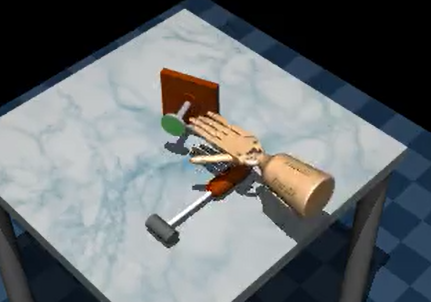
\includegraphics[width=1\linewidth]{C:/MGTU/baseAI/lr12/lr12/bag/report/images/begin.png}
        \caption*{а) Начало}
    \end{minipage}
    \hfill
    \begin{minipage}[H]{0.48\linewidth}
        \centering
        \includegraphics[width=0.99\linewidth]{C:/MGTU/baseAI/lr12/lr12/bag/report/images/took\_hammer.png}
        \caption*{б) Взятие молотка}
    \end{minipage}
    \caption{Визуализация работы агента 1}
    \label{fig:work1}
\end{figure}

\begin{figure}[H]
    \centering
    \begin{minipage}[H]{0.48\linewidth}
      \centering
      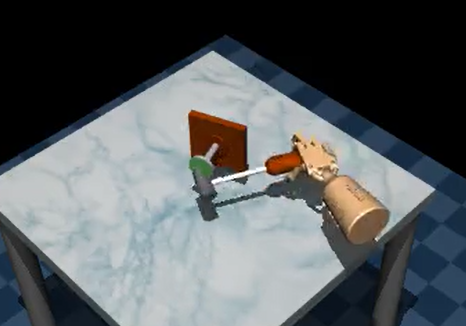
\includegraphics[width=80mm, height=60mm]{C:/MGTU/baseAI/lr12/lr12/bag/report/images/near_gvodz.png}
      \caption*{в) Молоток возле гвоздя}
    \end{minipage}
    \hfill
    \begin{minipage}[H]{0.48\linewidth}
      \centering
      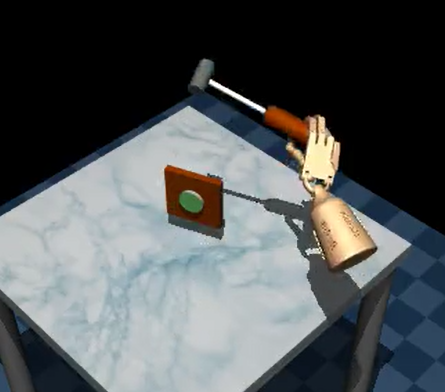
\includegraphics[width=80mm, height=60mm]{C:/MGTU/baseAI/lr12/lr12/bag/report/images/end.png}
      \caption*{г) Конец}
    \end{minipage}
    \caption{Визуализация работы агента 2}
    \label{fig:work2}
  \end{figure}

\section*{Вывод}

В ходе тестирования модель была успешно обучена на среде AdroitHandHammer-v1. 
Эта модель может быть использована для управления рукой-роботом, чтобы выполнить задачу забивания гвоздя.
График демонстрирует, что модель успешно вырабатывает эффективную стратегию для выполнения задачи, 
а рисунки демонстрируют, как агент успешно применяет полученную стратегию для выполнения задачи.

\clearpage
